\section{Trois 4-transposisitions}

\begin{theorem}
  All sggi of rank 4 on $A_{11}$ with three 4-transpositions are those displayed in appendix~\ref{rank4-3-4transpositions}
\end{theorem}

\begin{proof}
  Let, without loss of generaly, $\rho_1$ and $\rho_3$ be 4-transposition.

  \begin{figure}[H]
    \begin{center}
      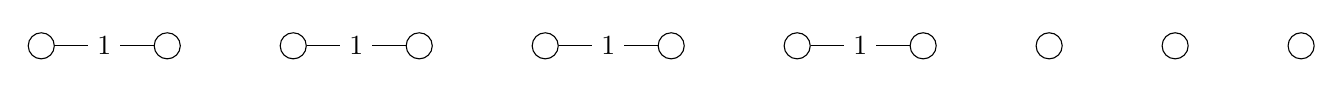
\begin{tikzpicture}[scale=.8]

        \begin{scope}[every node/.style={circle,draw}]
          \node (1)  at (0,0)  {};
          \node (2)  at (2,0)  {};
          \node (3)  at (4,0)  {};
          \node (4)  at (6,0)  {};
          \node (5)  at (8,0)  {};
          \node (6)  at (10,0)  {};
          \node (7)  at (12,0)  {};
          \node (8)  at (14,0)  {};
          \node (9)  at (16,0)  {};
          \node (10) at (18,0)  {};
          \node (11) at (20,0) {};
        \end{scope}

        \begin{scope}[every node/.style={fill=white}]

          \begin{scope}[every edge/.style={draw}]
            \path (1)  edge node {$1$} (2);
            \path (3)  edge node {$1$} (4);
            \path (5)  edge node {$1$} (6);
            \path (7)  edge node {$1$} (8);
          \end{scope}
        \end{scope}

      \end{tikzpicture}
      \caption{}
    \end{center}
  \end{figure}

  \paragraph{}~\footnote{TODO}


  \begin{figure}[H]
    \begin{center}
      \begin{tikzpicture}[scale=.8]

        \begin{scope}[every node/.style={circle,draw}]
          \node (1)  at (0,2)  {};
          \node (2)  at (0,0)  {};
          \node (3)  at (2,2)  {};
          \node (4)  at (2,0)  {};
          \node (5)  at (4,0)  {};
          \node (6)  at (6,0)  {};
          \node (7)  at (8,0)  {};
          \node (8)  at (10,0) {};
          \node (9)  at (12,0) {};
          \node (10) at (14,0) {};
          \node (11) at (16,0) {};
        \end{scope}

        \begin{scope}[every node/.style={fill=white}]

          \begin{scope}[every edge/.style={draw}]
            \path (1)  edge node {$1$} (2);
            \path (3)  edge node {$1$} (4);
            \path (5)  edge[bend right=30] node {$1$} (6);
            \path (7)  edge node {$1$} (8);
            \path (1)  edge node {$3$} (3);
            \path (2)  edge node {$3$} (4);
            \path (5)  edge[bend left=30] node {$3$} (6);
            \path (9)  edge node {$3$} (10);
          \end{scope}
        \end{scope}

      \end{tikzpicture}
      \caption{}
    \end{center}
  \end{figure}

  \paragraph{}
  Essayons de placer les involutions $\rho_0$, celles-ci doivent commuter avec $\rho_3$. On peut placer facilement un arête pour relier l'arête simple avec $\rho_1$ au point fixe. Mais pour l'autre c'est plus compliqué. Il faut trouver une arête $\rho_2$ unqiement contenue entre deux arêtes $\rho_1$. A priori, ça parait impossible mais en regardant bien, sur le carré alterne, nous avons deux cotés (les arêtes $\rho_3$) sont placées entre deux arêtes $\rho_1$. Mais ces arêtes ne sont pas $\rho_2$. On peut cependant rajouter une arête $\rho_2$ pour doubler l'arête $\rho_3$ et maintenant on peut la tripler avec $\rho_0$. On a donc

  \begin{figure}[H]
    \begin{center}
      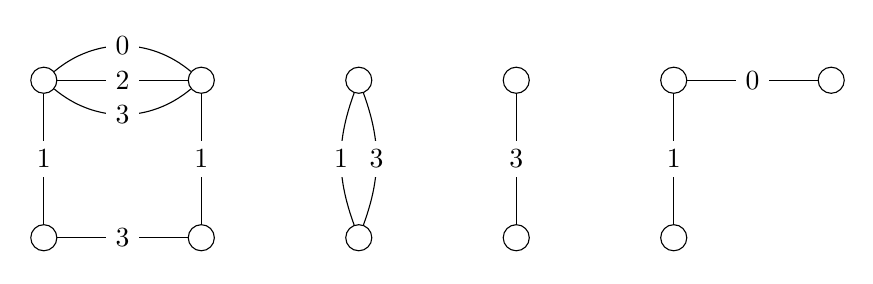
\begin{tikzpicture}

        \begin{scope}[every node/.style={circle,draw}]
          \node (1)  at (0,2)  {};
          \node (2)  at (0,0)  {};
          \node (3)  at (2,2)  {};
          \node (4)  at (2,0)  {};
          \node (5)  at (4,2)  {};
          \node (6)  at (4,0)  {};
          \node (7)  at (8,2)  {};
          \node (8)  at (8,0)  {};
          \node (9)  at (6,2)  {};
          \node (10) at (6,0)  {};
          \node (11) at (10,2) {};
        \end{scope}

        \begin{scope}[every node/.style={fill=white}]

          \begin{scope}[every edge/.style={draw}]
            \path (1)  edge[bend left=40] node {$0$} (3);
            \path (7)  edge node {$0$} (11);
            \path (1)  edge node {$1$} (2);
            \path (3)  edge node {$1$} (4);
            \path (5)  edge[bend right=20] node {$1$} (6);
            \path (7)  edge node {$1$} (8);
            \path (1)  edge node {$2$} (3);
            \path (1)  edge[bend right=40] node {$3$} (3);
            \path (2)  edge node {$3$} (4);
            \path (5)  edge[bend left=20] node {$3$} (6);
            \path (9)  edge node {$3$} (10);
          \end{scope}
        \end{scope}

      \end{tikzpicture}
      \caption{}
    \end{center}
  \end{figure}

  \paragraph{}
  Les trois dernières arêtes de $\rho_2$ doivent servir à relier les trois composantes connexes du graphe ci-dessus, sachant que l'arête 0 ne peut être relié à rien et qu'on ne sait créer que deux branches sur le carré alterné. Il y a donc 2 possibilités (une seule branche) plus 2 possibilités (deux branches, la branche avec $\rho_0$ ne contient aucune autre composante) plus 2 possibilités (deux branches, la branche avec $\rho_0$ contient deux composantes). On a donc exactement 6 possibilités.

\end{proof}
